\begin{enumerate}[label=\thesection.\arabic*.,ref=\thesection.\theenumi]
\numberwithin{equation}{enumi}
\item For a unity feedback system 
\begin{align}
G(s) = \frac{K}{(s)(s+2)(s+4)(s+6)}
\label{eq:ee18btech11046_system}
\end{align}
Design a lag compensator to yield a $K_{v}=2$ and Phase Margin of $30\degree$


\solution
%
\solution Fig.\ref{fig:ee18btech11046_flow} models the equivalent of compensated closed loop system. 
 \begin{figure}[!ht]
	\begin{center}
		\resizebox{\columnwidth}{!}{\begin{enumerate}[label=\thesection.\arabic*.,ref=\thesection.\theenumi]
\numberwithin{equation}{enumi}
\item For a unity feedback system 
\begin{align}
G(s) = \frac{K}{(s)(s+2)(s+4)(s+6)}
\label{eq:ee18btech11046_system}
\end{align}
Design a lag compensator to yield a $K_{v}=2$ and Phase Margin of $30\degree$


\solution
%
\solution Fig.\ref{fig:ee18btech11046_flow} models the equivalent of compensated closed loop system. 
 \begin{figure}[!ht]
	\begin{center}
		\resizebox{\columnwidth}{!}{\begin{enumerate}[label=\thesection.\arabic*.,ref=\thesection.\theenumi]
\numberwithin{equation}{enumi}
\item For a unity feedback system 
\begin{align}
G(s) = \frac{K}{(s)(s+2)(s+4)(s+6)}
\label{eq:ee18btech11046_system}
\end{align}
Design a lag compensator to yield a $K_{v}=2$ and Phase Margin of $30\degree$


\solution
%
\solution Fig.\ref{fig:ee18btech11046_flow} models the equivalent of compensated closed loop system. 
 \begin{figure}[!ht]
	\begin{center}
		\resizebox{\columnwidth}{!}{\begin{enumerate}[label=\thesection.\arabic*.,ref=\thesection.\theenumi]
\numberwithin{equation}{enumi}
\item For a unity feedback system 
\begin{align}
G(s) = \frac{K}{(s)(s+2)(s+4)(s+6)}
\label{eq:ee18btech11046_system}
\end{align}
Design a lag compensator to yield a $K_{v}=2$ and Phase Margin of $30\degree$


\solution
%
\solution Fig.\ref{fig:ee18btech11046_flow} models the equivalent of compensated closed loop system. 
 \begin{figure}[!ht]
	\begin{center}
		\resizebox{\columnwidth}{!}{\input{./figs/ee18btech11046.tex}}
	\end{center}
\caption{}
\label{fig:ee18btech11046_flow}
\end{figure}

%
Static Velocity Error Constant $K_{v}$ is the steady-state error of a system for a unit-ramp input i.e.,
\begin{align}
K_{v}=\lim _{s \rightarrow 0} s G(s) G_{c}(s)
\label{eq:ee18btech11046_compansatedsys}
\end{align}
Therefore,
\begin{multline}
K_{v}=\lim _{s \rightarrow 0} s \frac{K}{s(s+2)(s+4)(s+6)} \frac{Ts+1}{\beta Ts+1}
\\
\implies 
2 = \frac{K}{(0+2)(0+4)(0+6)} \frac{T(0)+1}{\beta T(0)+1}
\\
\therefore 
K = 96
\end{multline}
\begin{align}
G\brak{s}=\frac{96}{s(s+2)(s+4)(s+6)}
\label{eq:ee18btech11046_upsys}
\end{align}


\item The Magnitude and Phase response of G(s).\\
\solution Substituting $s = \j\omega$ in \eqref{eq:ee18btech11046_upsys},
\begin{multline}
G\brak{\j\omega} =\frac{96}{\brak{j\omega}\brak{j\omega+2}\brak{j\omega+4}\brak{j\omega+6}} 
\end{multline}
\begin{multline}
\abs{G\brak{\j\omega}} = \frac{\abs{96}}{\omega\sqrt{4+\omega^2}\sqrt{16+\omega^2}\sqrt{36+\omega^2}}
\label{eq:ee18btech11046_gain}
\end{multline}
\begin{multline}
\angle G\brak{\j\omega} = -90\degree -\tan^{-1}\brak{\frac{\omega}{2}}  - \tan^{-1}\brak{\frac{\omega}{4}} \\-  \tan^{-1}\brak{\frac{\omega}{6}} 
\label{eq:ee18btech11046_phase}
\end{multline}

\item The standard Transfer equation of Lag Compensator and its Phase and Gain\\
\solution
\begin{align}
G_{c}\brak{s} = \frac{Ts+1}{\beta Ts+1}
\label{eq:ee18btech11046_comp}
\\
\abs{G_{c}\brak{s}} = \frac{1}{\beta}\frac{1+\brak{\frac{\omega}{T}}^{2}}{1+\brak{\frac{\omega}{\beta T}}^{2}}
\label{eq:ee18btech11046_compGain}
\\
\angle G_{c}\brak{s} = \tan^{-1}\brak{\omega T}-\tan^{-1}\brak{\omega \beta T}
\label{eq:ee18btech11046_compPhase}
\end{align}
Where $\beta > 1$.

It can be approximated that for $\omega > \frac{1}{T}$  
\begin{align}
\abs{G_{c}\brak{s}} = \frac{1}{\beta}
\label{eq:ee18btech11046_compGainapprox}
\end{align}
and Phase to be very small($<12\degree$).


\item The Phase Margin(PM) of the Transfer function G(s)\\
\solution
From \eqref{eq:ee18btech11046_gain} and \eqref{eq:ee18btech11046_gain}

At Gain Crossover,
\begin{align}
\abs{G\brak{s}} = 1
\\
\implies
\omega_{gc} = 1.47rad/sec
\\
\implies
\angle G\brak{\j \omega_{gc}} = -160.26\degree
\end{align}
\begin{align}
PM = 180\degree + \angle G\brak{\j \omega_{gc}}
\\
\implies
PM = 19.74\degree
\end{align}
The following are the Bode plots of uncompensated system
\begin{figure}[!h]
\centering
  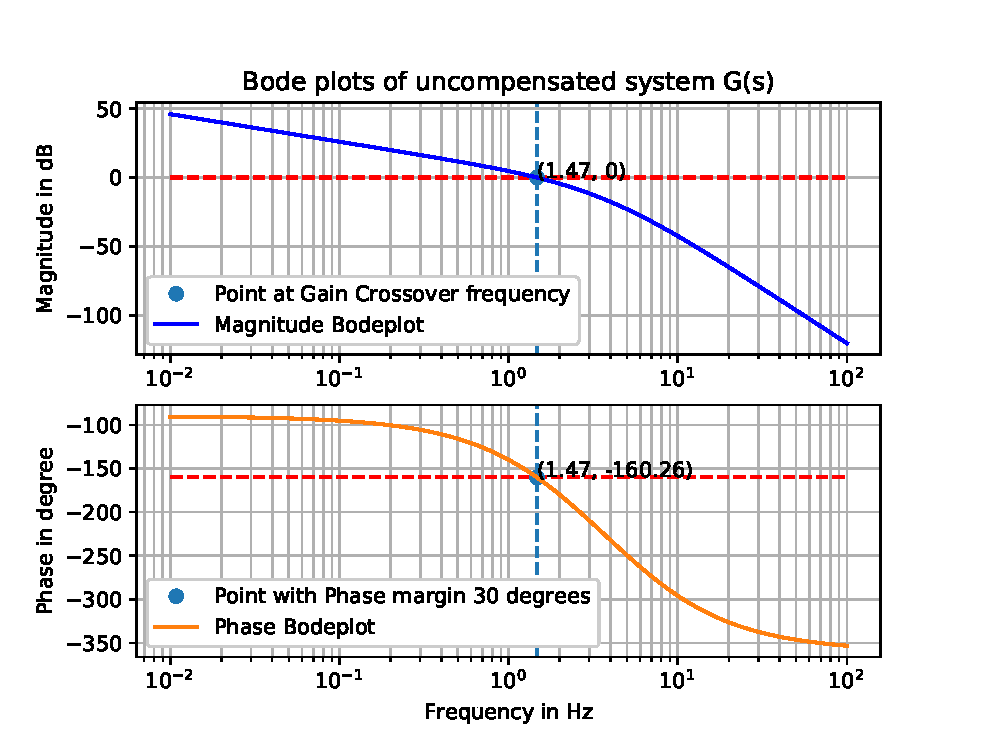
\includegraphics[width=\columnwidth]{./figs/ee18btech11046_1.eps}
\caption{}
\label{fig:ee18btech11046_uncompensated} 
\end{figure}
%

The code for Bode plots of uncompensated system 
\begin{lstlisting}
codes/ee18btech11046_1.py
\end{lstlisting}
% 



\item Design a lag compansator such that the Phase Margin becomes $30\degree$ \\
\solution
The lag compansator form is given in  \eqref{eq:ee18btech11046_comp},
Let
\begin{align}
G^{'}\brak{s}=G\brak{s}G_{c}\brak{s}
\end{align}
The $PM = 30\degree$ when $\angle G^{'}\brak{\j\omega} = -150\degree$ 

Since the addition of compensator reduces Gain of system, thereby reducing Gain Crossover frequency which increases Phase Margin(PM) of system.

Since, Compansator also has small negative phase(say $\epsilon$),let $\epsilon =5\degree$.i.e, $\angle G_{c}\brak{s} = 5$ 
\begin{align}
\angle G^{'}\brak{s} = \angle G\brak{s} + \angle G_{c}\brak{s}
\\
\implies
-150\degree = \angle G\brak{s} - 5\degree
\\
\implies
\angle G\brak{s} = -145\degree
\end{align}
The value of $\omega$ where $\angle G\brak{s} = -145\degree$ is 
\begin{align}
\angle G\brak{s} = -145\degree
\\
\implies
\omega_{req} = 1.10953rad/sec
\label{eq:ee18b46_omega-req}
\end{align}
The value $\frac{1}{T}$ is exactly 2 octaves below $\omega_{req}$ obtained in \eqref{eq:ee18b46_omega-req}
\begin{align}
\frac{1}{T} = \frac{\omega_{req}}{4}
\\
\implies
T = 3.605
\label{eq:ee18btech11046_T}
\end{align}
Now we should take $\beta$ such that Gain Crossover frequency occurs at $\omega_{req}$ i.e., to make $\abs{G^{'}\brak{\j\omega}} = 1$

From \eqref{eq:ee18btech11046_compGainapprox},

\begin{align}
\abs{G^{'}\brak{\j\omega_{gc}}} = \abs{G\brak{\j\omega_{gc}}}\abs{G_{c}\brak{\j\omega_{gc}}} = 1
\\
\implies
1.4936 \times \frac{1}{\beta} = 1
\\
\implies
\beta = 1.4936
\label{eq:ee18btech11046_beta}
\end{align} 
Substituting values of T and $\beta$ obtained from\eqref{eq:ee18btech11046_T} and\eqref{eq:ee18btech11046_beta} in \eqref{eq:ee18btech11046_comp}
The required Compensator Transfer is
\begin{align}
G_{c}\brak{s} = \frac{3.605s+1}{5.384s+1}
\end{align}
The following are the Bode plots of compensated system
\begin{figure}[!h]
\centering
  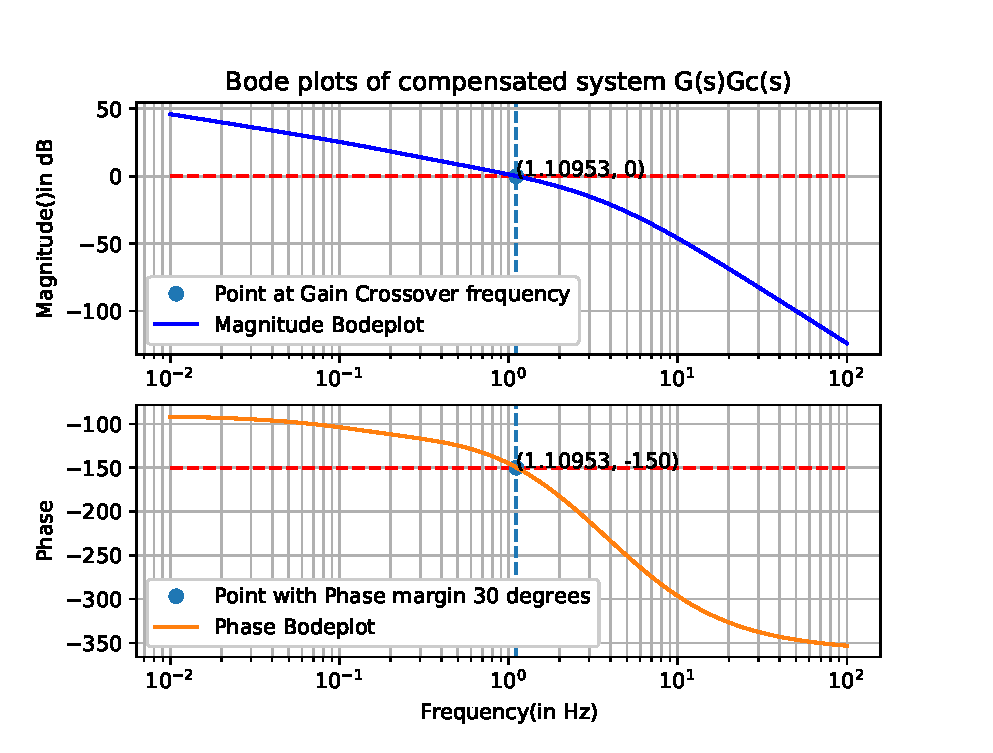
\includegraphics[width=\columnwidth]{./figs/ee18btech11046_2.eps}
\caption{}
\label{fig:ee18btech11046_compensated} 
\end{figure}
%

The code for Bode plots of compensated system 
\begin{lstlisting}
codes/ee18btech11046_2.py
\end{lstlisting}
% 

\end{enumerate}
}
	\end{center}
\caption{}
\label{fig:ee18btech11046_flow}
\end{figure}

%
Static Velocity Error Constant $K_{v}$ is the steady-state error of a system for a unit-ramp input i.e.,
\begin{align}
K_{v}=\lim _{s \rightarrow 0} s G(s) G_{c}(s)
\label{eq:ee18btech11046_compansatedsys}
\end{align}
Therefore,
\begin{multline}
K_{v}=\lim _{s \rightarrow 0} s \frac{K}{s(s+2)(s+4)(s+6)} \frac{Ts+1}{\beta Ts+1}
\\
\implies 
2 = \frac{K}{(0+2)(0+4)(0+6)} \frac{T(0)+1}{\beta T(0)+1}
\\
\therefore 
K = 96
\end{multline}
\begin{align}
G\brak{s}=\frac{96}{s(s+2)(s+4)(s+6)}
\label{eq:ee18btech11046_upsys}
\end{align}


\item The Magnitude and Phase response of G(s).\\
\solution Substituting $s = \j\omega$ in \eqref{eq:ee18btech11046_upsys},
\begin{multline}
G\brak{\j\omega} =\frac{96}{\brak{j\omega}\brak{j\omega+2}\brak{j\omega+4}\brak{j\omega+6}} 
\end{multline}
\begin{multline}
\abs{G\brak{\j\omega}} = \frac{\abs{96}}{\omega\sqrt{4+\omega^2}\sqrt{16+\omega^2}\sqrt{36+\omega^2}}
\label{eq:ee18btech11046_gain}
\end{multline}
\begin{multline}
\angle G\brak{\j\omega} = -90\degree -\tan^{-1}\brak{\frac{\omega}{2}}  - \tan^{-1}\brak{\frac{\omega}{4}} \\-  \tan^{-1}\brak{\frac{\omega}{6}} 
\label{eq:ee18btech11046_phase}
\end{multline}

\item The standard Transfer equation of Lag Compensator and its Phase and Gain\\
\solution
\begin{align}
G_{c}\brak{s} = \frac{Ts+1}{\beta Ts+1}
\label{eq:ee18btech11046_comp}
\\
\abs{G_{c}\brak{s}} = \frac{1}{\beta}\frac{1+\brak{\frac{\omega}{T}}^{2}}{1+\brak{\frac{\omega}{\beta T}}^{2}}
\label{eq:ee18btech11046_compGain}
\\
\angle G_{c}\brak{s} = \tan^{-1}\brak{\omega T}-\tan^{-1}\brak{\omega \beta T}
\label{eq:ee18btech11046_compPhase}
\end{align}
Where $\beta > 1$.

It can be approximated that for $\omega > \frac{1}{T}$  
\begin{align}
\abs{G_{c}\brak{s}} = \frac{1}{\beta}
\label{eq:ee18btech11046_compGainapprox}
\end{align}
and Phase to be very small($<12\degree$).


\item The Phase Margin(PM) of the Transfer function G(s)\\
\solution
From \eqref{eq:ee18btech11046_gain} and \eqref{eq:ee18btech11046_gain}

At Gain Crossover,
\begin{align}
\abs{G\brak{s}} = 1
\\
\implies
\omega_{gc} = 1.47rad/sec
\\
\implies
\angle G\brak{\j \omega_{gc}} = -160.26\degree
\end{align}
\begin{align}
PM = 180\degree + \angle G\brak{\j \omega_{gc}}
\\
\implies
PM = 19.74\degree
\end{align}
The following are the Bode plots of uncompensated system
\begin{figure}[!h]
\centering
  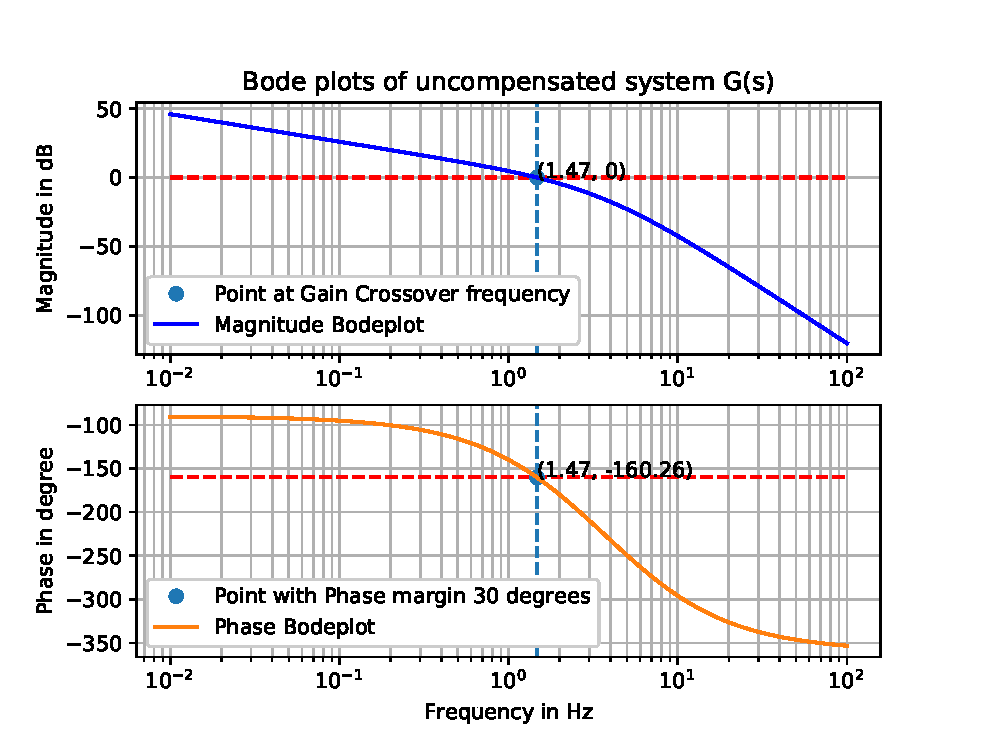
\includegraphics[width=\columnwidth]{./figs/ee18btech11046_1.eps}
\caption{}
\label{fig:ee18btech11046_uncompensated} 
\end{figure}
%

The code for Bode plots of uncompensated system 
\begin{lstlisting}
codes/ee18btech11046_1.py
\end{lstlisting}
% 



\item Design a lag compansator such that the Phase Margin becomes $30\degree$ \\
\solution
The lag compansator form is given in  \eqref{eq:ee18btech11046_comp},
Let
\begin{align}
G^{'}\brak{s}=G\brak{s}G_{c}\brak{s}
\end{align}
The $PM = 30\degree$ when $\angle G^{'}\brak{\j\omega} = -150\degree$ 

Since the addition of compensator reduces Gain of system, thereby reducing Gain Crossover frequency which increases Phase Margin(PM) of system.

Since, Compansator also has small negative phase(say $\epsilon$),let $\epsilon =5\degree$.i.e, $\angle G_{c}\brak{s} = 5$ 
\begin{align}
\angle G^{'}\brak{s} = \angle G\brak{s} + \angle G_{c}\brak{s}
\\
\implies
-150\degree = \angle G\brak{s} - 5\degree
\\
\implies
\angle G\brak{s} = -145\degree
\end{align}
The value of $\omega$ where $\angle G\brak{s} = -145\degree$ is 
\begin{align}
\angle G\brak{s} = -145\degree
\\
\implies
\omega_{req} = 1.10953rad/sec
\label{eq:ee18b46_omega-req}
\end{align}
The value $\frac{1}{T}$ is exactly 2 octaves below $\omega_{req}$ obtained in \eqref{eq:ee18b46_omega-req}
\begin{align}
\frac{1}{T} = \frac{\omega_{req}}{4}
\\
\implies
T = 3.605
\label{eq:ee18btech11046_T}
\end{align}
Now we should take $\beta$ such that Gain Crossover frequency occurs at $\omega_{req}$ i.e., to make $\abs{G^{'}\brak{\j\omega}} = 1$

From \eqref{eq:ee18btech11046_compGainapprox},

\begin{align}
\abs{G^{'}\brak{\j\omega_{gc}}} = \abs{G\brak{\j\omega_{gc}}}\abs{G_{c}\brak{\j\omega_{gc}}} = 1
\\
\implies
1.4936 \times \frac{1}{\beta} = 1
\\
\implies
\beta = 1.4936
\label{eq:ee18btech11046_beta}
\end{align} 
Substituting values of T and $\beta$ obtained from\eqref{eq:ee18btech11046_T} and\eqref{eq:ee18btech11046_beta} in \eqref{eq:ee18btech11046_comp}
The required Compensator Transfer is
\begin{align}
G_{c}\brak{s} = \frac{3.605s+1}{5.384s+1}
\end{align}
The following are the Bode plots of compensated system
\begin{figure}[!h]
\centering
  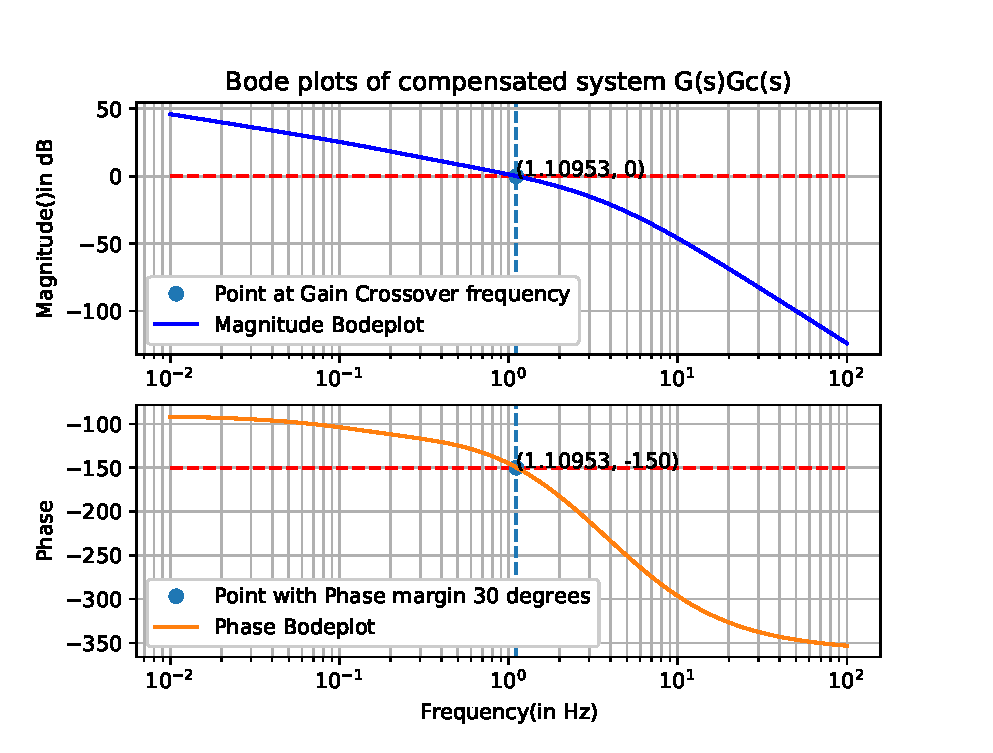
\includegraphics[width=\columnwidth]{./figs/ee18btech11046_2.eps}
\caption{}
\label{fig:ee18btech11046_compensated} 
\end{figure}
%

The code for Bode plots of compensated system 
\begin{lstlisting}
codes/ee18btech11046_2.py
\end{lstlisting}
% 

\end{enumerate}
}
	\end{center}
\caption{}
\label{fig:ee18btech11046_flow}
\end{figure}

%
Static Velocity Error Constant $K_{v}$ is the steady-state error of a system for a unit-ramp input i.e.,
\begin{align}
K_{v}=\lim _{s \rightarrow 0} s G(s) G_{c}(s)
\label{eq:ee18btech11046_compansatedsys}
\end{align}
Therefore,
\begin{multline}
K_{v}=\lim _{s \rightarrow 0} s \frac{K}{s(s+2)(s+4)(s+6)} \frac{Ts+1}{\beta Ts+1}
\\
\implies 
2 = \frac{K}{(0+2)(0+4)(0+6)} \frac{T(0)+1}{\beta T(0)+1}
\\
\therefore 
K = 96
\end{multline}
\begin{align}
G\brak{s}=\frac{96}{s(s+2)(s+4)(s+6)}
\label{eq:ee18btech11046_upsys}
\end{align}


\item The Magnitude and Phase response of G(s).\\
\solution Substituting $s = \j\omega$ in \eqref{eq:ee18btech11046_upsys},
\begin{multline}
G\brak{\j\omega} =\frac{96}{\brak{j\omega}\brak{j\omega+2}\brak{j\omega+4}\brak{j\omega+6}} 
\end{multline}
\begin{multline}
\abs{G\brak{\j\omega}} = \frac{\abs{96}}{\omega\sqrt{4+\omega^2}\sqrt{16+\omega^2}\sqrt{36+\omega^2}}
\label{eq:ee18btech11046_gain}
\end{multline}
\begin{multline}
\angle G\brak{\j\omega} = -90\degree -\tan^{-1}\brak{\frac{\omega}{2}}  - \tan^{-1}\brak{\frac{\omega}{4}} \\-  \tan^{-1}\brak{\frac{\omega}{6}} 
\label{eq:ee18btech11046_phase}
\end{multline}

\item The standard Transfer equation of Lag Compensator and its Phase and Gain\\
\solution
\begin{align}
G_{c}\brak{s} = \frac{Ts+1}{\beta Ts+1}
\label{eq:ee18btech11046_comp}
\\
\abs{G_{c}\brak{s}} = \frac{1}{\beta}\frac{1+\brak{\frac{\omega}{T}}^{2}}{1+\brak{\frac{\omega}{\beta T}}^{2}}
\label{eq:ee18btech11046_compGain}
\\
\angle G_{c}\brak{s} = \tan^{-1}\brak{\omega T}-\tan^{-1}\brak{\omega \beta T}
\label{eq:ee18btech11046_compPhase}
\end{align}
Where $\beta > 1$.

It can be approximated that for $\omega > \frac{1}{T}$  
\begin{align}
\abs{G_{c}\brak{s}} = \frac{1}{\beta}
\label{eq:ee18btech11046_compGainapprox}
\end{align}
and Phase to be very small($<12\degree$).


\item The Phase Margin(PM) of the Transfer function G(s)\\
\solution
From \eqref{eq:ee18btech11046_gain} and \eqref{eq:ee18btech11046_gain}

At Gain Crossover,
\begin{align}
\abs{G\brak{s}} = 1
\\
\implies
\omega_{gc} = 1.47rad/sec
\\
\implies
\angle G\brak{\j \omega_{gc}} = -160.26\degree
\end{align}
\begin{align}
PM = 180\degree + \angle G\brak{\j \omega_{gc}}
\\
\implies
PM = 19.74\degree
\end{align}
The following are the Bode plots of uncompensated system
\begin{figure}[!h]
\centering
  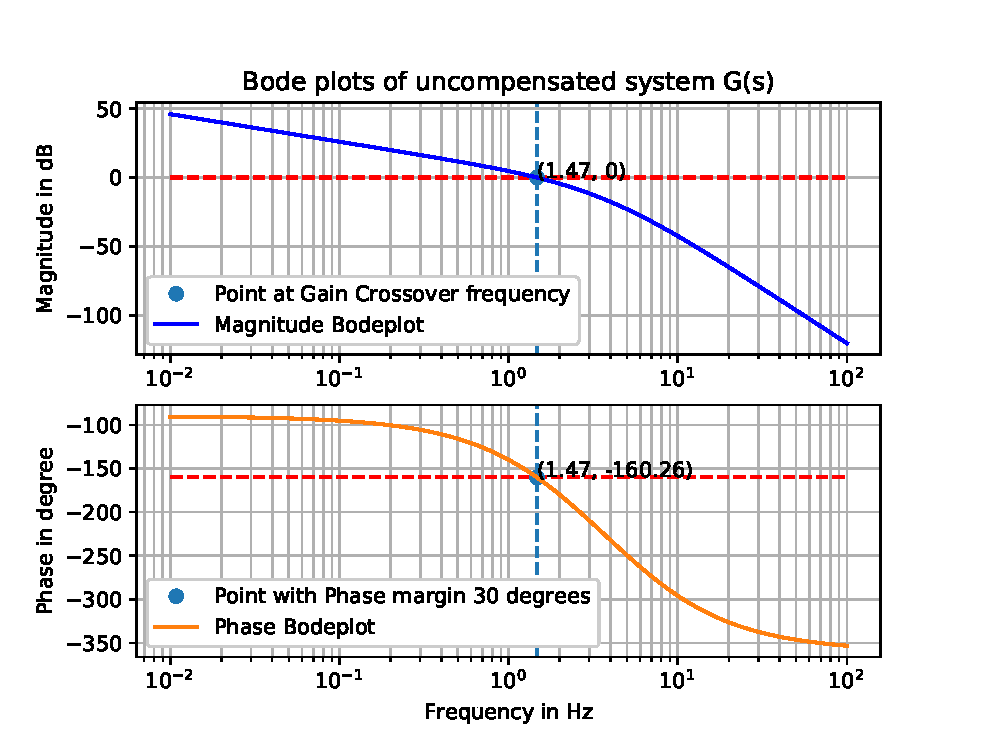
\includegraphics[width=\columnwidth]{./figs/ee18btech11046_1.eps}
\caption{}
\label{fig:ee18btech11046_uncompensated} 
\end{figure}
%

The code for Bode plots of uncompensated system 
\begin{lstlisting}
codes/ee18btech11046_1.py
\end{lstlisting}
% 



\item Design a lag compansator such that the Phase Margin becomes $30\degree$ \\
\solution
The lag compansator form is given in  \eqref{eq:ee18btech11046_comp},
Let
\begin{align}
G^{'}\brak{s}=G\brak{s}G_{c}\brak{s}
\end{align}
The $PM = 30\degree$ when $\angle G^{'}\brak{\j\omega} = -150\degree$ 

Since the addition of compensator reduces Gain of system, thereby reducing Gain Crossover frequency which increases Phase Margin(PM) of system.

Since, Compansator also has small negative phase(say $\epsilon$),let $\epsilon =5\degree$.i.e, $\angle G_{c}\brak{s} = 5$ 
\begin{align}
\angle G^{'}\brak{s} = \angle G\brak{s} + \angle G_{c}\brak{s}
\\
\implies
-150\degree = \angle G\brak{s} - 5\degree
\\
\implies
\angle G\brak{s} = -145\degree
\end{align}
The value of $\omega$ where $\angle G\brak{s} = -145\degree$ is 
\begin{align}
\angle G\brak{s} = -145\degree
\\
\implies
\omega_{req} = 1.10953rad/sec
\label{eq:ee18b46_omega-req}
\end{align}
The value $\frac{1}{T}$ is exactly 2 octaves below $\omega_{req}$ obtained in \eqref{eq:ee18b46_omega-req}
\begin{align}
\frac{1}{T} = \frac{\omega_{req}}{4}
\\
\implies
T = 3.605
\label{eq:ee18btech11046_T}
\end{align}
Now we should take $\beta$ such that Gain Crossover frequency occurs at $\omega_{req}$ i.e., to make $\abs{G^{'}\brak{\j\omega}} = 1$

From \eqref{eq:ee18btech11046_compGainapprox},

\begin{align}
\abs{G^{'}\brak{\j\omega_{gc}}} = \abs{G\brak{\j\omega_{gc}}}\abs{G_{c}\brak{\j\omega_{gc}}} = 1
\\
\implies
1.4936 \times \frac{1}{\beta} = 1
\\
\implies
\beta = 1.4936
\label{eq:ee18btech11046_beta}
\end{align} 
Substituting values of T and $\beta$ obtained from\eqref{eq:ee18btech11046_T} and\eqref{eq:ee18btech11046_beta} in \eqref{eq:ee18btech11046_comp}
The required Compensator Transfer is
\begin{align}
G_{c}\brak{s} = \frac{3.605s+1}{5.384s+1}
\end{align}
The following are the Bode plots of compensated system
\begin{figure}[!h]
\centering
  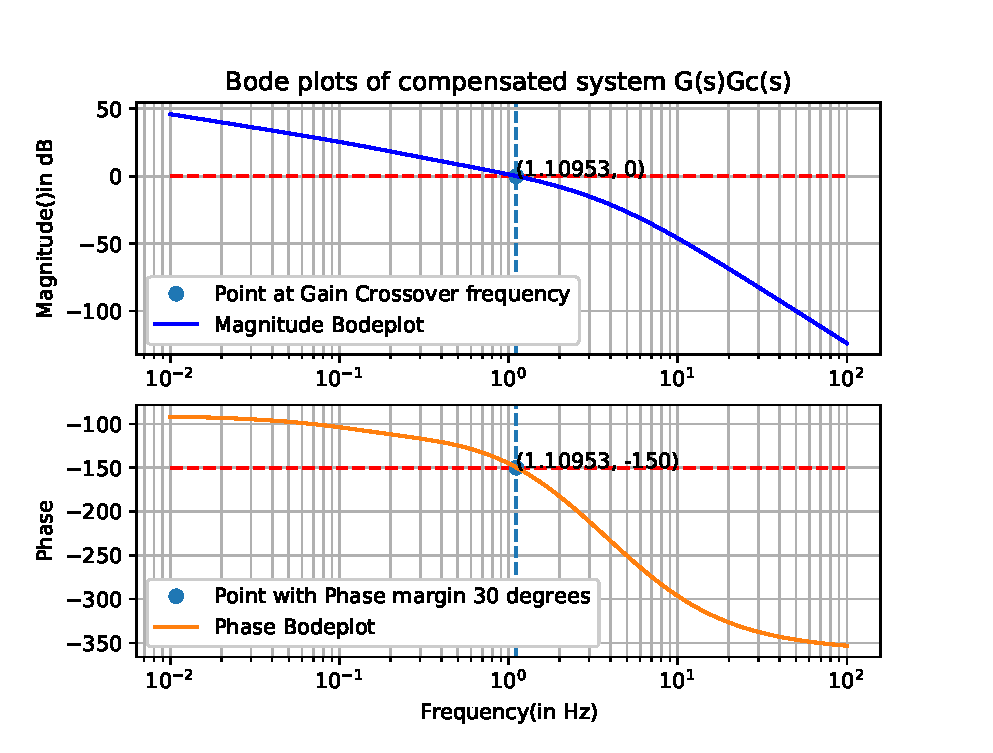
\includegraphics[width=\columnwidth]{./figs/ee18btech11046_2.eps}
\caption{}
\label{fig:ee18btech11046_compensated} 
\end{figure}
%

The code for Bode plots of compensated system 
\begin{lstlisting}
codes/ee18btech11046_2.py
\end{lstlisting}
% 

\end{enumerate}
}
	\end{center}
\caption{}
\label{fig:ee18btech11046_flow}
\end{figure}

%
Static Velocity Error Constant $K_{v}$ is the steady-state error of a system for a unit-ramp input i.e.,
\begin{align}
K_{v}=\lim _{s \rightarrow 0} s G(s) G_{c}(s)
\label{eq:ee18btech11046_compansatedsys}
\end{align}
Therefore,
\begin{multline}
K_{v}=\lim _{s \rightarrow 0} s \frac{K}{s(s+2)(s+4)(s+6)} \frac{Ts+1}{\beta Ts+1}
\\
\implies 
2 = \frac{K}{(0+2)(0+4)(0+6)} \frac{T(0)+1}{\beta T(0)+1}
\\
\therefore 
K = 96
\end{multline}
\begin{align}
G\brak{s}=\frac{96}{s(s+2)(s+4)(s+6)}
\label{eq:ee18btech11046_upsys}
\end{align}


\item The Magnitude and Phase response of G(s).\\
\solution Substituting $s = \j\omega$ in \eqref{eq:ee18btech11046_upsys},
\begin{multline}
G\brak{\j\omega} =\frac{96}{\brak{j\omega}\brak{j\omega+2}\brak{j\omega+4}\brak{j\omega+6}} 
\end{multline}
\begin{multline}
\abs{G\brak{\j\omega}} = \frac{\abs{96}}{\omega\sqrt{4+\omega^2}\sqrt{16+\omega^2}\sqrt{36+\omega^2}}
\label{eq:ee18btech11046_gain}
\end{multline}
\begin{multline}
\angle G\brak{\j\omega} = -\frac{\pi}{2} -\tan^{-1}\brak{\frac{\omega}{2}}  - \tan^{-1}\brak{\frac{\omega}{4}} - \tan^{-1}\brak{\frac{\omega}{6}} 
\label{eq:ee18btech11046_phase}
\end{multline}

\item The standard Transfer equation of Lag Compensator and its Phase and Gain\\
\solution
\begin{align}
G_{c}\brak{s} = \frac{Ts+1}{\beta Ts+1}
\label{eq:ee18btech11046_comp}
\\
\abs{G_{c}\brak{s}} = \frac{1}{\beta}\frac{1+\brak{\frac{\omega}{T}}^{2}}{1+\brak{\frac{\omega}{\beta T}}^{2}}
\label{eq:ee18btech11046_compGain}
\\
\angle G_{c}\brak{s} = \tan^{-1}\brak{\omega T}-\tan^{-1}\brak{\omega \beta T}
\label{eq:ee18btech11046_compPhase}
\end{align}
Where $\beta > 1$.

It can be approximated that for $\omega > \frac{1}{T}$  
\begin{align}
\abs{G_{c}\brak{s}} = \frac{1}{\beta}
\label{eq:ee18btech11046_compGainapprox}
\end{align}
and Phase to be very small($<12\degree$).


\item The Phase Margin(PM) of the Transfer function G(s)\\
\solution
From \eqref{eq:ee18btech11046_gain} and \eqref{eq:ee18btech11046_gain}

At Gain Crossover,
\begin{align}
\abs{G\brak{s}} = 1
\\
\implies
\omega_{gc} = 1.47rad/sec
\\
\implies
\angle G\brak{\j \omega_{gc}} = -160.26\degree
\end{align}
\begin{align}
PM = 180\degree + \angle G\brak{\j \omega_{gc}}
\\
\implies
PM = 19.74\degree
\end{align}
The following are the Bode plots of uncompensated system
\begin{figure}[!h]
\centering
  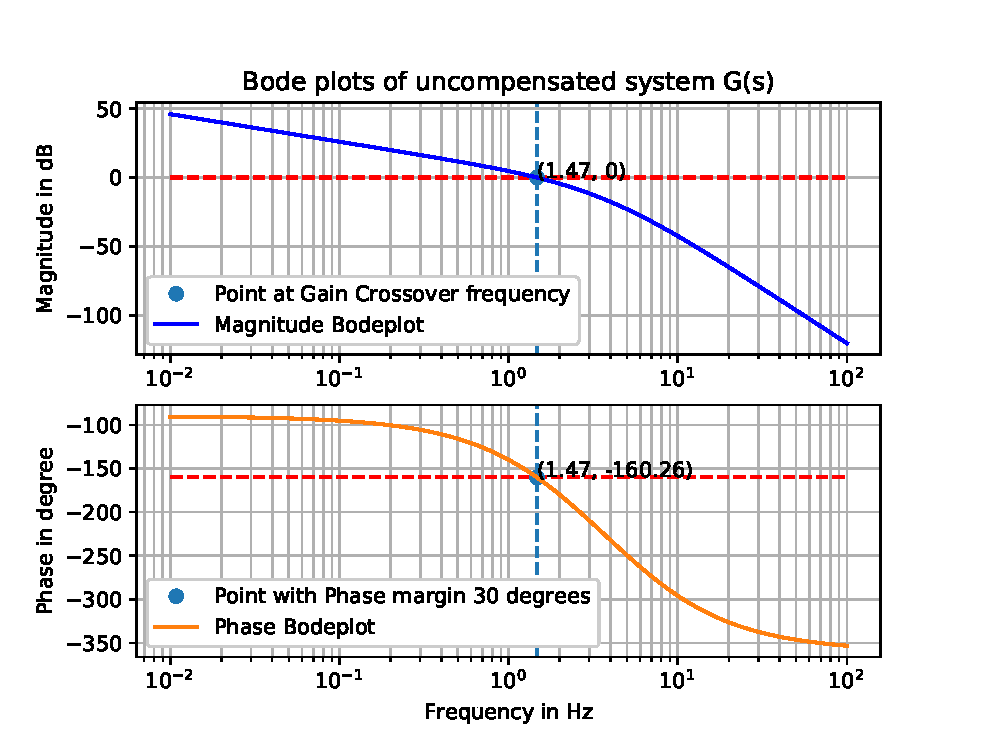
\includegraphics[width=\columnwidth]{./figs/ee18btech11046_1.eps}
\caption{}
\label{fig:ee18btech11046_uncompensated} 
\end{figure}
%

The code for Bode plots of uncompensated system 
\begin{lstlisting}
codes/ee18btech11046_1.py
\end{lstlisting}
% 



\item Design a lag compansator such that the Phase Margin becomes $30\degree$ \\
\solution
The lag compansator form is given in  \eqref{eq:ee18btech11046_comp},
Let
\begin{align}
G^{'}\brak{s}=G\brak{s}G_{c}\brak{s}
\end{align}
The $PM = 30\degree$ when $\angle G^{'}\brak{\j\omega} = -150\degree$ 

Since the addition of compensator reduces Gain of system, thereby reducing Gain Crossover frequency which increases Phase Margin(PM) of system.

Since, Compansator also has small negative phase(say $\epsilon$),let $\epsilon =5\degree$.i.e, $\angle G_{c}\brak{s} = 5$ 
\begin{align}
\angle G^{'}\brak{s} = \angle G\brak{s} + \angle G_{c}\brak{s}
\\
\implies
-150\degree = \angle G\brak{s} - 5\degree
\\
\implies
\angle G\brak{s} = -145\degree
\end{align}
The value of $\omega$ where $\angle G\brak{s} = -145\degree$ is 
\begin{align}
\angle G\brak{s} = -145\degree
\\
\implies
\omega_{req} = 1.10953rad/sec
\label{eq:ee18b46_omega-req}
\end{align}
The value $\frac{1}{T}$ is exactly 2 octaves below $\omega_{req}$ obtained in \eqref{eq:ee18b46_omega-req}
\begin{align}
\frac{1}{T} = \frac{\omega_{req}}{4}
\\
\implies
T = 3.605
\label{eq:ee18btech11046_T}
\end{align}
Now we should take $\beta$ such that Gain Crossover frequency occurs at $\omega_{req}$ i.e., to make $\abs{G^{'}\brak{\j\omega}} = 1$

From \eqref{eq:ee18btech11046_compGainapprox},

\begin{align}
\abs{G^{'}\brak{\j\omega_{gc}}} = \abs{G\brak{\j\omega_{gc}}}\abs{G_{c}\brak{\j\omega_{gc}}} = 1
\\
\implies
1.4936 \times \frac{1}{\beta} = 1
\\
\implies
\beta = 1.4936
\label{eq:ee18btech11046_beta}
\end{align} 
Substituting values of T and $\beta$ obtained from\eqref{eq:ee18btech11046_T} and\eqref{eq:ee18btech11046_beta} in \eqref{eq:ee18btech11046_comp}
The required Compensator Transfer is
\begin{align}
G_{c}\brak{s} = \frac{3.605s+1}{5.384s+1}
\end{align}
The following are the Bode plots of compensated system
\begin{figure}[!h]
\centering
  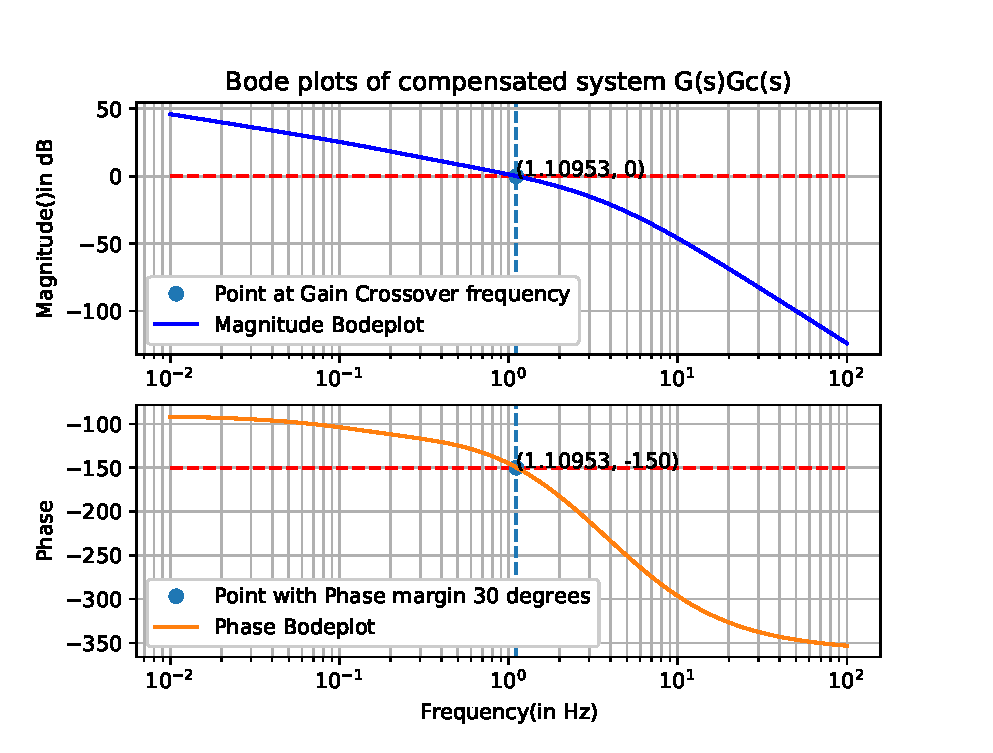
\includegraphics[width=\columnwidth]{./figs/ee18btech11046_2.eps}
\caption{}
\label{fig:ee18btech11046_compensated} 
\end{figure}
%

The code for Bode plots of compensated system 
\begin{lstlisting}
codes/ee18btech11046_2.py
\end{lstlisting}
% 

\end{enumerate}
